% Chaptre 1

\chapter{Etat de l’art} % Main chapter title

\label{Chaptre3} % For referencing the chapter elsewhere, use \ref{Chapter1} 

Dans cette partie je vais  présenter le positionnement des mes missions par rapport à l’état de l’art scientifique ou technique.
\section{Le cloud computing}
Le cloud computing ou informatique en nuage est une infrastructure dans laquelle la puissance de calcul et le stockage sont gérés par des serveurs distants auxquels les usagers se connectent via une liaison Internet sécurisée.\\ \\ L'ordinateur de bureau ou portable, le téléphone mobile, la tablette tactile et autres objets connectés deviennent des points d'accès pour exécuter des applications ou consulter des données qui sont hébergées sur les serveurs. \\ \\ Le cloud se caractérise également par sa souplesse qui permet aux fournisseurs d'adapter automatiquement la capacité de stockage et la puissance de calcul aux besoins des utilisateurs.\\ \\
Comme illustration, le cloud computing se matérialise notamment par les services de stockage et de partage de données numériques type Box, Dropbox, Microsoft OneDrive ou Apple iCloud sur lesquels les utilisateurs peuvent stocker des contenus personnels (photos, vidéos, musique, documents...) et y accéder n'importe où dans le monde depuis n'importe quel terminal connecté.
 \begin{figure}[H]
            \centering
                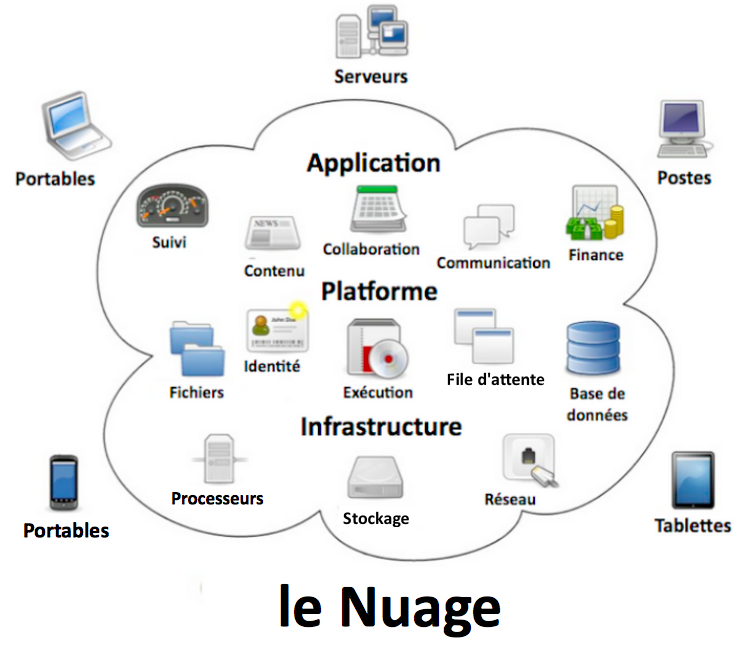
\includegraphics[width=0.5\textwidth]{Figures/cloud}
	       \decoRule
		\caption[Le Cloud]{Le Cloud}
	\label{fig:Cloud}
	\end{figure}
\subsection{Les services du cloud computing} On distingue plusieurs types de services cloud \\
\subsubsection{IaaS (Infrastructure as a Service, en anglais) }
C'est un modèle du cloud computing où l'entreprise dispose sur abonnement payant d'une infrastructure informatique (serveurs, stockage, sauvegarde, réseau) qui se trouve physiquement chez le fournisseur qui est aussi responsable pour la sécurité de l'infrastructure.\\ \\Cela peut représenter pour certaines directions des systèmes d’information (DSI) un moyen de réaliser des économies, principalement en transformant des investissements en contrats de location.

\subsubsection{PaaS (Platform as a Service, en anglais)}
C'est un  modèle du cloud computing qui permet de mettre à disposition des entités clientes un environnement d'exécution rapidement disponible, en leur laissant la maîtrise des applications qu'elles peuvent installer, configurer et utiliser elles-mêmes.\\ \\ Il se distingue ainsi du modèle SaaS où la même application est mise à disposition des nombreux utilisateurs finaux
\subsubsection{SaaS (Software as a Service, en anglais)}
C'est un modèle du cloud computing qui fournit des applications  sous forme de services clés en mains auxquels les utilisateurs se connectent via des logiciels dédiés ou un navigateur Internet. \\ \\Exemple Les service de messageries électroniques type Gmail, Yahoo, Outlook.com ou de suites bureautiques type Office 365 ou Google Apps.
\newpage
\section{Les APIs(Application programming interface)}
une API est une façade clairement délimitée par laquelle une application offre des services à d’autres applications. Cette façade peut comporter des classes, des méthodes ou des fonctions, des types de données et
des constantes. Les API peuvent être publiques, partenaires ou privées
 \begin{figure}[H]
            \centering
                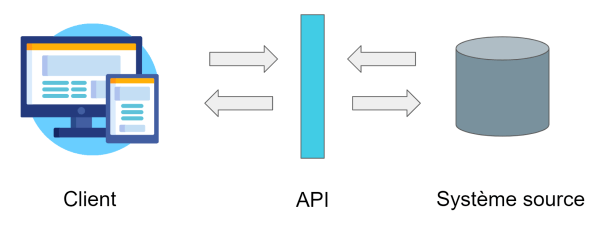
\includegraphics[width=0.8\textwidth]{Figures/api}
	       \decoRule
		\caption[API]{API}
	\label{fig:api}
	\end{figure}
\subsection{Objectif d’une API}
Tout comme une interface utilisateur graphique facilite l’utilisation des programmes pour les profanes, une
API a pour objectif de fournir une porte d’accès à une ou plusieurs fonctionnalités d’un système en exposant
uniquement les objets ou les actions dont le développeur a besoin et en cachant les détails de la mise en
œuvre. Elles permettent ainsi aux développeurs d’utiliser plus facilement certaines technologies pour créer
des applications. Une API simplifie la programmation.



\subsection{Analogie d’une API avec la vie courante}

Prenons l’exemple d’un appel téléphonique, la plupart des gens ne savent pas comment se déroule un appel
téléphonique : le mécanisme électronique qui régit un appel téléphonique. Pourtant tout le monde peut
effectuer un appel juste en composant le numéro de son correspondant et en appuyant simplement sur
un bouton (envoyer ou ok) du clavier. Le clavier et l’écran du téléphone sont l’équivalent de l’API; ils
représentent l’interface du système électronique qui régit un appel téléphonique

\section{Le modèle ou l'architecture Rest}
Les APIs peuvent être intégrées suivant plusieurs modèles ou styles d’architecture : le modèle à base des
simples fonctions, le modèle RPC, le modèle SOAP, le modèle Rest puis le modèle GraphQL.
Le modèle Rest, est un style orienté ressources et utilisant principalement le protocole HTTP pour la communication. Avec le modèle Rest les données entre le client et le fournisseur sont transmises en format JSON ou
XML. Ainsi, Rest utilise des notions qu’il faut obligatoirement comprendre : les ressources, les identifiants, les méthodes HTTP, et les formats de données.
\subsection{Les principes de l’architecture REST}
L'architecture Rest est régit par six principes suivants:
\begin{enumerate}
	\item La séparation entre client et serveur\\
les responsabilités du côté serveur et du côté client sont
séparées, si bien que chaque côté peut être implémenté indépendamment de l’autre. Le code
côté serveur (l’API) et celui côté client peuvent chacun être modifiés sans affecter l’autre, tant
que tous deux continuent de communiquer dans le même format. Dans une architecture REST,
différents clients envoient des requêtes sur les mêmes endpoints, effectuent les mêmes actions et
obtiennent les mêmes réponses.
     \item . L’absence d’état de sessions (stateless)\\
la communication entre client et serveur ne conserve pas
l’état des sessions d’une requête à l’autre. Autrement dit, l’état d’une session est inclus dans
chaque requête, ce qui signifie que ni le client ni le serveur n’a besoin de connaître l’état de
l’autre pour communiquer. Chaque requête est complète et se suffit à elle-même : pas besoin de maintenir une connexion continue entre client et serveur, ce qui implique une plus
grande tolérance à l’échec. De plus, cela permet aux APIs REST de répondre aux requêtes
de plusieurs clients différents sans saturer les ports du serveur. L’exception à cette règle est
l’authentification, pour que le client n’ait pas à préciser ses informations d’authentification à
chaque requête.
      \item L’uniformité de l’interface\\
les différentes actions et/ou ressources disponibles avec leurs endpoints et leurs paramètres spécifiques doivent être décidés et respectés religieusement, de façon
uniforme par le client et le serveur. Chaque réponse doit contenir suffisamment d’informations
pour être interprétée sans que le client n’ait besoin d’autres informations au préalable. Les
réponses ne doivent pas être trop longues et doivent contenir, si nécessaire, des liens vers d’autres
endpoints. 
       \item La mise en cache\\
les réponses peuvent être mises en cache pour éviter de surcharger inutilement le serveur. La mise en cache doit être bien gérée : l’API REST doit préciser si telle ou telle
réponse peut être mise en cache et pour combien de temps pour éviter que le client ne reçoive
des informations obsolètes.
        \item L’architecture en couches\\
un client connecté à une API REST ne peut en général pas distinguer
s’il est en communication avec le serveur final ou un serveur intermédiaire. Une architecture
REST permet par exemple de recevoir les requêtes sur un serveur A, de stocker ses données sur
un serveur B et de gérer les authentifications sur un serveur C.
        \item Le code à la demande
Cette contrainte est optionnelle. Elle signifie qu’une API peut retourner
du code exécutable au lieu d’une réponse en \textbf{JSON} ou en XML par exemple. Cela signifie qu’une
API \textbf{RESTful} peut étendre le code du client tout en lui simplifiant la vie en lui fournissant du
code exécutable tel qu’un script \textbf{JavaScript}.

\end{enumerate}

Une API REST ne peut être qualifiée de \textbf{RESTful} si elle ne respecte pas les six contraintes, mais on peut
tout de même la qualifier d’API REST si elle n’enfreint que deux ou trois principes. REST est sans doute le
standard le plus utilisé pour concevoir des architectures d’API, mais il en existe bien d’autres qui pourraient le complémenter, voire un jour le détrôner

\section{L’architecture serverless}
C’est une architecture où l’utilisateur n’a pas à gérer la moindre infrastructure. L’architecture serverless ne signifie pas pour autant qu’il n’y a pas de serveurs : cela veut dire qu’ils sont invisibles pour l’utilisateur et sont gérés par les fournisseurs et non par les consommateurs. Sans trop penser à leur maintenance, les ressources informatiques sont utilisées comme des services.
 
L’architecture serverless fait changer la façon dont on conçoit et maintient les applications. Elle permet aux consommateurs de bâtir des plateformes en utilisant exclusivement des services managés, de se concentrer sur les aspects liés à la logique business, et non sur les contraintes de déploiement ou de scalabilité.
\begin{list}{•}
	\item  Exemples fournisseur des architectures Serverless
	\begin{itemize}
		\item AWS
		\begin{list}{*}
			\item Amazon S3
			\item Amazon Dynamodb
			\item Amazon Lambda
        \end{list}
		\item Google:
		\begin{list}{*}
			\item Google Cloud Functions
		\end{list}
		\item Microsoft
		\begin{list}{*}
			\item Azure Functions
		\end{list}
	\end{itemize}

\end{list}


%----------------------------------------------------------------------------------------

\section{Le protocole OAuth2 et la délégation d’autorisation}

Le Oauth2 est la seconde version du protocole Oauth(Open Autorization). Connu comme protocole de
délégation d’autorisations, le Oauth2 est un protocole qui permet à une application d’obtenir une autorisation d’accès limitée aux ressources disponibles sur un serveur accessible via HTTP. Si ces ressources
n’appartiennent pas à l’application, l’autorisation d’accès lui est déléguée par le détenteur des ressources ;
au cas contraire l’application obtient l’autorisation en s’authentifiant avec ses identifiants. Avec le protocole Oauth2 le propriétaire de ressources ne partage pas ses identifiants avec l’application qui sollicite ses
ressources. Le protocole Oauth2 fournit un modèle dans lequel le détenteur de ressource peut accorder un
accès limité à ses données en émettant simplement un jeton temporaire, qui sera utilisé par cette application
sollicitant ses données pour s’identifier auprès du serveur de ressources. Le protocole Oauth2 met le propriétaire de ressources au cœur du système d’octroi d’autorisation. C’est le propriétaire de ressources qui
fait le lien entre ses comptes sur différentes applications sans que des administrateurs de la sécurité aient
besoin d’intervenir directement sur chaque application.

\subsection{Exemple d’implémentation du protocole Oauth2}

Le protocole Oauth2 est utilisé par plusieurs entreprises comme Facebook, Google et Twitter. L’exemple que nous proposons ici est celui qui permet
d’afficher instantanément les tweets sur Facebook sans avoir besoin de votre mot de passe Facebook
\newpage
\subsection{Le vocabulaire du protocole Oauth2}
\textbf{Les rôles}: Le protocole Oauth2 identifie quatre rôles: Client, Propriétaire de ressources, Serveur d’autorisation
et Serveur de ressources.
\begin{list}{•}
	\item  Le détenteur des ressources(Resource Owner):\\
	 Le détenteur ou le propriétaire de ressources est
	une entité capable d’accorder l’accès à une ressource protégée. Lorsque le propriétaire de la ressource est une personne, on parle d’ utilisateur final.

	\item Le serveur de ressources (Resource Server):\\
	Le serveur de ressources est le serveur qui héberge
	les ressources protégées ou à accès limité. Un exemple du serveur des ressources peut être Facebook et Google qui hébergent les informations des profils des utilisateurs.
	\item Le client (Client Application): \\
	C’est une application qui sollicite les ressources du serveur de
	ressources, celle-ci peut être une application PHP, une application mobile, une application Javascript.
	\item Le serveur d’autorisation (Authorization Server):\\
	Le serveur d’autorisation représente le serveur
	qui délivre des jetons au client. Ces jetons seront utilisés lors des requêtes du client vers le serveur de ressources. Ce serveur peut être le même que le serveur de ressources (physiquement et applicativement), et c’est souvent le cas.
\end{list}
\textbf{Les jetons:} Un jeton est une chaîne des caractères, générée par le serveur d’autorisation au client une fois
qu’ une autorisation lui est offerte.
\begin{list}{•}
	\item Le jeton d’accès(Access token):\\
	 est un jeton nécessaire pour accéder aux ressources partagées par
	OAuth2. Il a une durée de vie qui est généralement assez courte.
	\item  
	\item Le jeton de renouvellement (Refresh Token):\\
	 est un jeton que le serveur d’autorisation peut émettre aux clients et il peut être échangé contre un nouveau jeton d’accès, sans répéter le processus d’autorisation. Il n’a pas de temps d’expiration.
\end{list}

\textbf{Les types d’autorisations(Grant types)}

\begin{list}{•}
	\item L’autorisation implicite (Implicit Grant): \\
	Elle doit être utilisée quand l’application se trouve côté
	client(typiquement une application Javascript). Il ne permet pas d’obtenir de token de renouvellement.
	
	\begin{figure}[H]
            \centering
                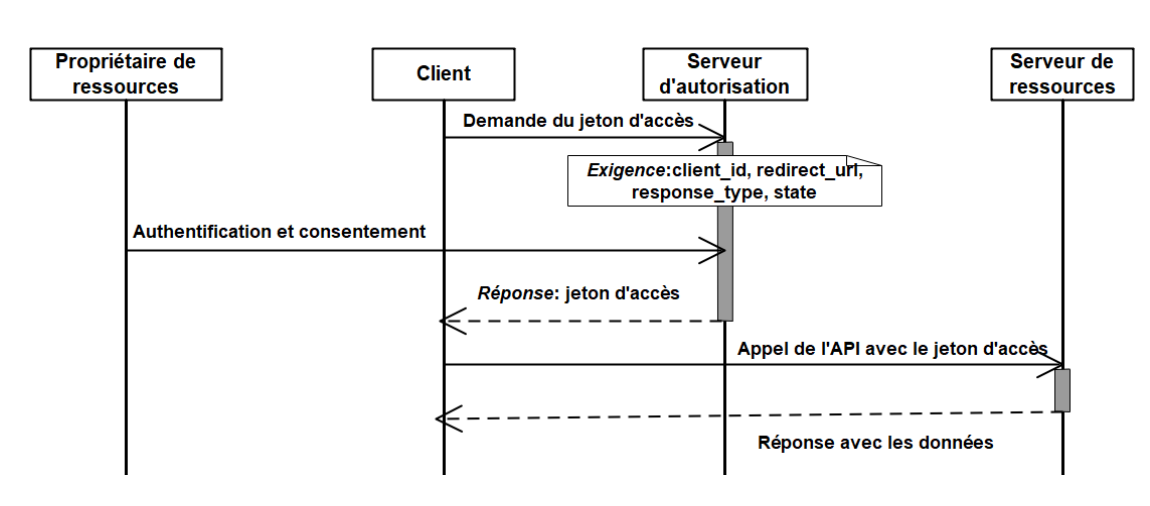
\includegraphics[width=0.8\textwidth]{Figures/implicit_grant}
	       \decoRule
		\caption[Implicit grant]{Implicit grant}
	\label{fig:implicit}
	\end{figure}
	\newpage
	\item L’autorisation via un code (Authorization Code Grant): \\
	Ce type d’autorisation permet d’obtenir deux jetons : le jeton d’accès et le jeton de renouvellement. Le client dans ce cas de figure interagit
	avec le propriétaire des ressources via un client web généralement un navigateur
	\begin{figure}[H]
            \centering
                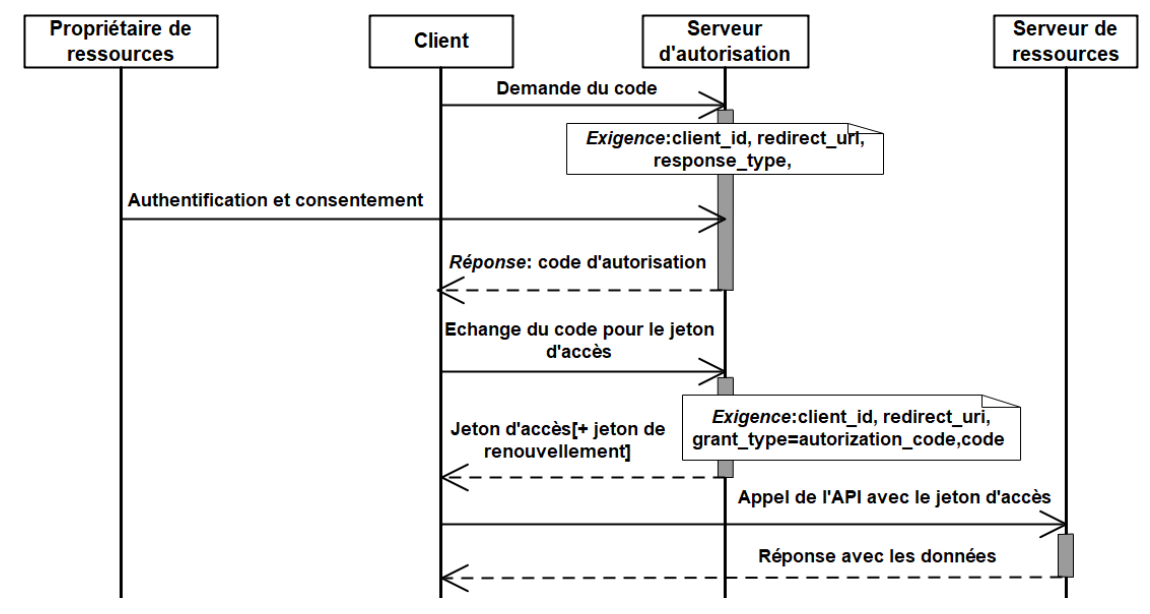
\includegraphics[width=0.8\textwidth]{Figures/code_grant}
	       \decoRule
		\caption[Code grant]{Code grant}
	\label{fig:Code}
	\end{figure}
	
	\item L’autorisation serveur à serveur (Client Credentials Grant):\\
	 Elle doit être utilisée lorsque le client est lui-même le détenteur des données. Il n’y a pas d’autorisation à obtenir de la part de l’utilisateur
	 \begin{figure}[H]
            \centering
                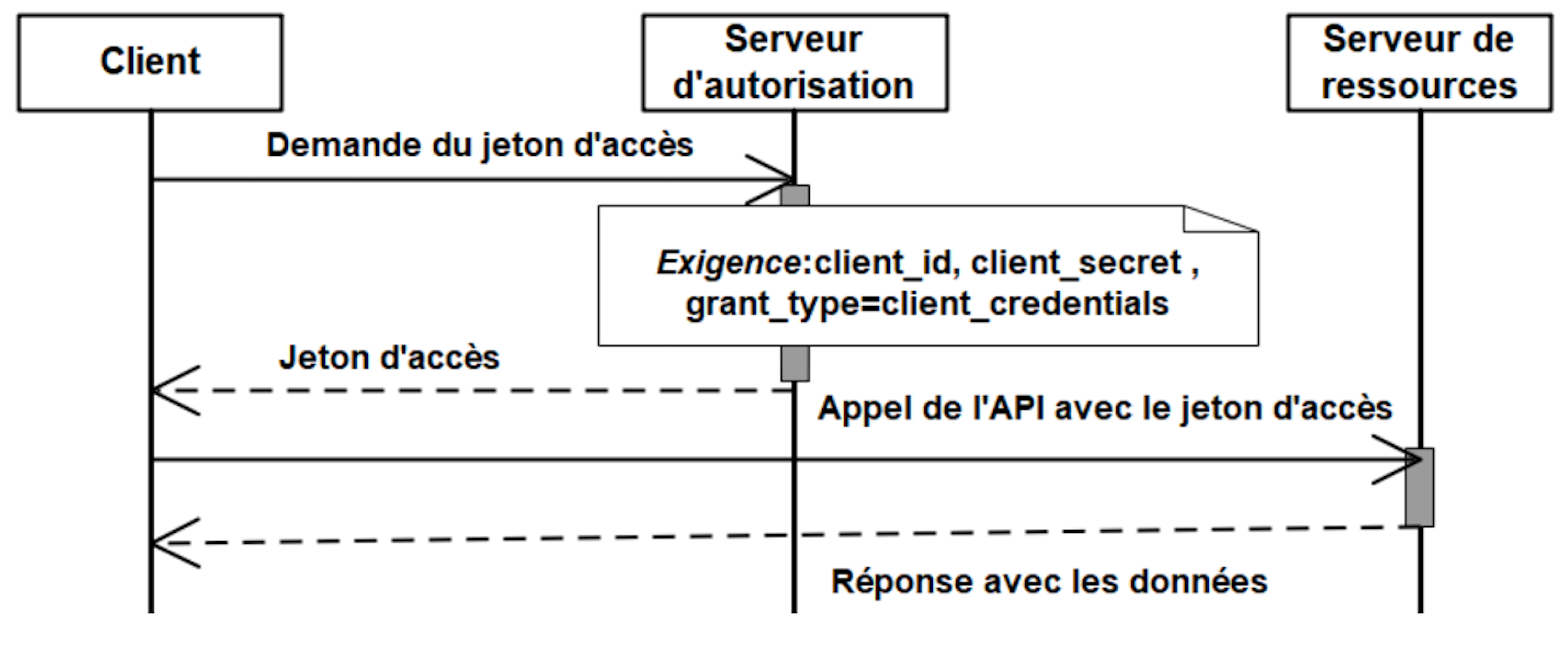
\includegraphics[width=0.8\textwidth]{Figures/server_server}
	       \decoRule
		\caption[Sever grant]{Server grant}
	\label{fig:Server}
	\end{figure}
	\newpage
	 \item L’autorisation via mot de passe (Resource Owner Password Credentials Grant):\\
	 Avec ce type d’autorisation, les identifiants sont envoyés au client et ensuite au serveur d’autorisation. Il est donc
	 impératif qu’il y ait une confiance absolue entre ces 2 entités. Ce type d’autorisation est principalement utilisé lorsque le client a été développé par la même autorité que celle          fournissant le serveur d’autorisation final.
	 \begin{figure}[H]
            \centering
                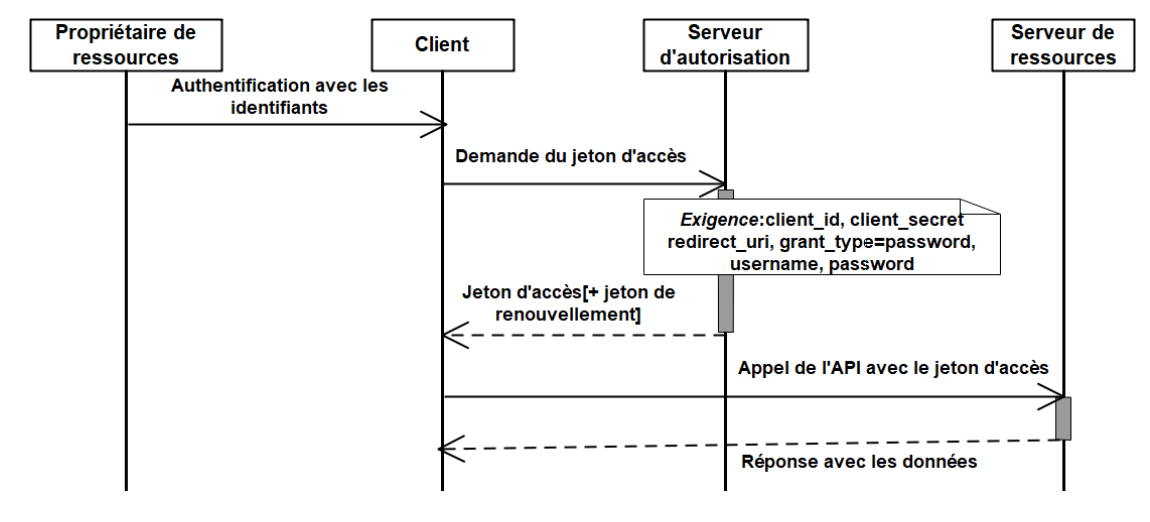
\includegraphics[width=0.8\textwidth]{Figures/password_grant}
	       \decoRule
		\caption[Password grant]{Password grant}
	\label{fig:Password}
	\end{figure}
\end{list}

\newpage
%----------------------------------------------------------------------------------------
\section{Intégration de données}
L’intégration des données est le processus qui consiste à combiner des données provenant de différentes
sources dans une vue unifiée : de l’importation au nettoyage en passant par le mapping et la transformation dans un gisement cible, pour finalement rendre les données plus exploitables et plus utiles pour les
utilisateurs qui les consultent.
\subsection{Les avantages}
\begin{list}{•}
	\item L’intégration des données améliore l’unification des systèmes et la collaboration globale
	\item L’intégration des données fait gagner du temps
	\item L’intégration des données réduit les erreurs (et les besoins de modifications)
\end{list}
\subsection{Opérations ETL et intégration des données}
Les opérations d’extraction, de transformation et de chargement (ETL) forment un processus d’intégration
à part entière dans lequel les données sont extraites du système source et livrées au data warehouse. Il s’agit
d’un processus continu que le data warehousing exécute pour transformer plusieurs sources de données en
informations cohérentes et utiles destinées à la Business Intelligence et aux analyses.
 \begin{figure}[H]
            \centering
                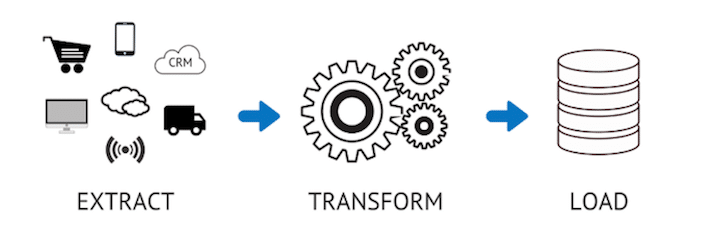
\includegraphics[width=0.8\textwidth]{Figures/etl}
	       \decoRule
		\caption[ETL]{ETL}
	\label{fig:ETL}
	\end{figure}
\newpage
\section{Conteneurisation}
Un conteneur est un système qui permet de stocker et d’isoler des objets devant être transportés ou déployés dans un environnement d’exploitation étendu (applications, logiciels, librairie, etc.). Il permet également au code applicatif d’être transporté de l’environnement de développement vers celui de production de manière aisée et sûre.  
La conteneurisation permet:
%La conteneurisation permet 

\begin{list}{•}
	\item De virtualiser, à l’intérieur d’un conteneur les ressources matérielles dont une application a besoin pour être exécutée(mémoire, réseau, processeur, etc.) 
	\item
	\item D'embarquer les composants logiciels nécessaires à l’application (données, fichiers, etc.)  
\end{list}

La conteneurisation est parfois confondue avec la virtualisation. Quand la première nécessite que chaque machine virtuelle possède 
son système d’exploitation, les conteneurs eux se connectent au noyau des machines, kernel, pour en exploiter les ressources. 
Moins lourds, ils sont plus faciles à déplacer et à stocker. 
 \begin{figure}[H]
            \centering
                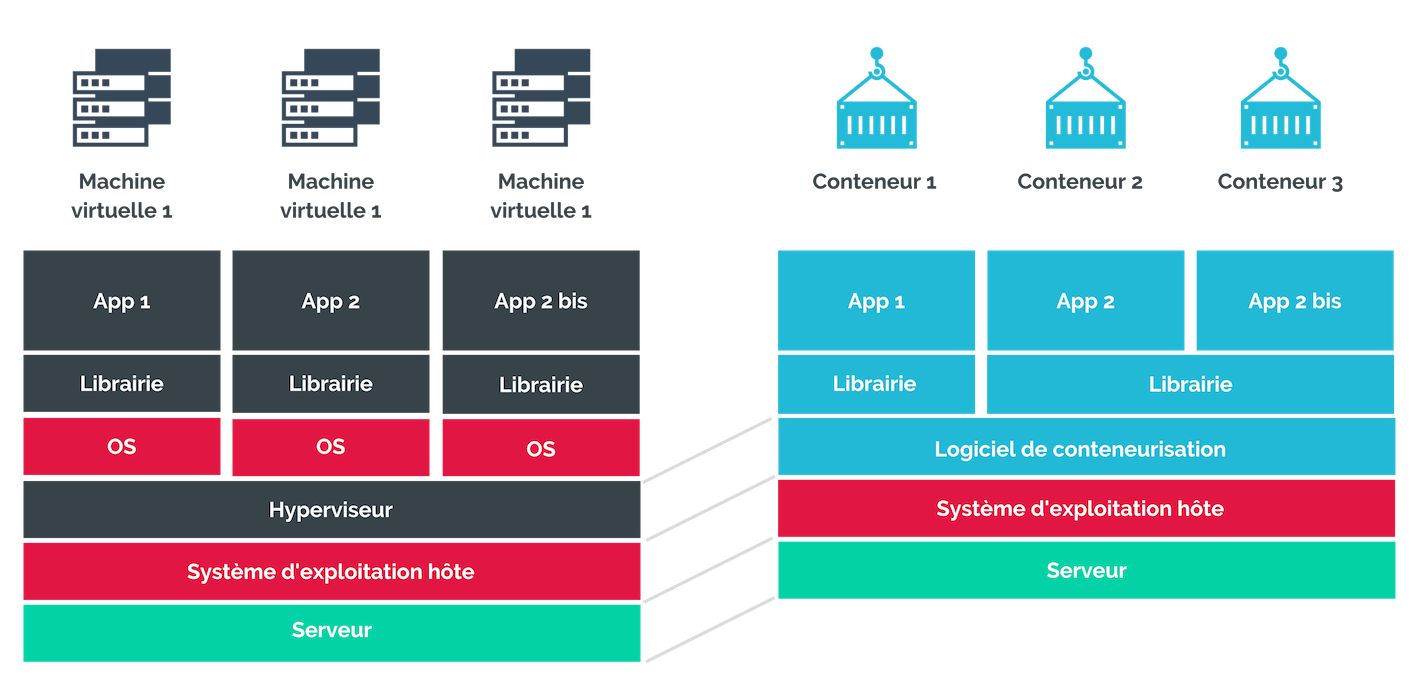
\includegraphics[width=0.8\textwidth]{Figures/virtualvscont}
	       \decoRule
		\caption[VM vs Conteneurisation]{VM vs Conteneurisation}
   \label{fig:VM vs Conteneurisation}
\end{figure}
%link : https://codalis.ch/conteneurisation-docker/

%Il s’agit d’un type de virtualisation utilisé au niveau des applications. Le principe repose sur la création de
%plusieurs espaces utilisateurs isolés les uns des autres sur un noyau commun. On utilise alors le terme de
%« conteneur » pour désigner une telle instance. Cette séparation repose sur un concept similaire à celui des
%modules applicatifs cloisonnés, communiquant à l’aide de services et applications web. Les conteneurs,
%bien qu’ indépendants, partagent un noyau commun (donc un ou plusieurs systèmes d’exploitation) et un
%même espace mémoire.
%La conteneurisation permet de packager tous les services, scripts, API, librairies dont une application a
%besoin. L’objectif : en permettre l’exécution sur n’importe quel noyau compatible
\subsection{Avantages}
\begin{list}{•}
	\item Elle évite de se soucier d’interactions ou d’incompatibilités avec les conteneurs déjà présents ou à
	venir sur cette machine.
	\item 
	\item Elle permet de ne pas occuper autant de ressources que réclamerait une machine virtuelle (ou virtual machine, VM), qui emporte son propre système d’exploitation et bloque des ressources à son
	lancement.
\end{list}
\subsection{Exemple des systèmes de conteneurisation}
\begin{list}{•}
	\item Docker
	\item Kubernetes
	\item CoreOs rkt
	\item OpenV
\end{list}
